\documentclass{school-22.101-notes}
\date{September 14, 2011}

\begin{document}
\maketitle

\subtopic{Postulate 2}
\hi{The state function/state is a wave function that contains all knowledge pertained to that particle}
A quantum state $\psi(\uline{x}, t)$ is complex in space and time, is normalized, and contains all knowledge (aka any physical behavior associated with the state) we may be interested in learning about the physical behavior. 

\subtopic{Postulate 3} 
\hi{Probabilities of measurement values can be found using postulate 1 \& 2}
Given an observable A, we find the operator $\hat{A}$, and the corresponding eigenvalues $a_i$ through $\hat{A} u_i = a_i u_i$. Then the probability of measuring the i-th eigenvalue is:
\eqn{ P(a_i) = |C_i|^2 }
in which $C_i$ is the expansion coefficient of $\psi(\uline{x}, t)$ with eigenfunction of $\hat{A}$. 

The completeness property of eigenfunctions tells us that we can expand the quantum state with a linear superposition of its eigenfunctions:
\begin{align}
\psi(\uline{x}) &= \Sum C_i u_i (\uline{x}) \\
C_i &= \int \dV u_i^* (\uline{x}) \psi(\uline{x}) = \mbox{Probability Amplitude}
\end{align}

Given the observable or the operator, we can solve for the eigenfunctions. Then if we also know the state function, we can solve for the expansion coefficient, and then the probability associated with each eigenvalues. This is what we mean in Law 2 that the state function contains all the information (aka knowing it we can solve for everything else). 

\uline{Example: Probability for position measurements} 
\eqn{ C_j = \int \dx \delta (x-x_j) \psi(x) = \psi(x_j) }
\eqn{ \Rightarrow P(x_j) = |\psi(x_j)|^2  }
This is suggesting that the probability of finding a particle between 0 and L is the highest at L/2. This expression is right, except that the probably at an exact point in the space is actually ill-defined, so the probability of position measurement should really be:
\eqn{ \boxed{ P(x \to x + \dx) \dx = |\psi(x_j)|^2 \dx  } }
The probability has to add up to 1: 
\eqn{ \int_{-\infty}^{\infty} P(x \to x +\dx) \dx = 1 = \int_{-\infty}^{\infty} |\psi(x)|^2 \dx  }
This suggests, again, that the state function has to be normalized. 

\uline{Example: Probability for momentum measurements}
Normalization problem of the eigenfunction:
\begin{align}
|\psi (x)|^2 &= \int |A|^2 e^{-ikx} e^{ik^{\prime}x} \dx = \int |A|^2 e^{i(k^{\prime}-k)x} = \delta(k^{\prime} - k) = \left\{ \begin{array}{cc}  1 & k^{\prime} = k  \\ 0 &  k^{\prime} \neq k   \end{array} \right. \\
\Rightarrow A &= \frac{1}{\sqrt{2 \pi}}  \\
 C_k &= \int  u_k^*(x) \psi(x) \dx = \int  A^* e^{-ikx} \psi(x) \dx = \sqrt{2 \pi} \Phi(k) A^* = \Phi(k)
\end{align}
in which we use Fourier transform of function represented in variable $x$ into an outcome of $k$:
\eqn{ \Phi(k) = \frac{1}{\sqrt{2\pi}} \int \dx e^{-ikx} \psi(x)  }
Similarly, we can use the inverse FT:
\eqn{ \psi(x) = \Sum C_k u_k (x) = \int C_k u_k(x) \dx = \int \Phi(k) \frac{1}{\sqrt{2\pi}} e^{ikx} \dx }
That is to say, $\psi(x), \Phi(k)$ carry the same information, just with different variables. 


\uline{Summary of Probabilities}
The two examples we've done so far are the common probabilities:
\eqn{ \boxed{ P(x \to x+\dx) \dx = |\psi(x)|^2 \dx = \mbox{wavefunction itself} } }
\eqn{ \boxed{ P(\hbar(k \to k + \dk) ) \dk = |\Phi(k)|^2 \dk = \mbox{F.T. of wavefunction}  }}

\uline{Energy Eigenvalue Problem, 1D, particle in a box}
We are given a box with the potential:
\eqn{ V(x) = \left\{ \begin{array}{cc} 0 & 0 \le x \le L \\ \infty & x<0, x>L  \end{array} \right. }
So there are infinite potential walls at location x=0 and x=L. Then we can immediately know the boundary conditions should be: $\psi_n (0) = 0, \psi_n(L) = 0$. 

Answer: We divide the problem into two parts:
\begin{enumerate}
\item Outside: 
\eqn{ \hat{H} = \frac{\hat{p}^2}{2m} + V = \infty }
\item Inside: 
\eqn{ \hat{H} = \frac{\hat{p}^2}{2m} + V = \frac{\hat{p}^2}{2m} }
\eqn{ -\frac{\hbar^2}{2m} \ppxn2 \psi_n = E_n \psi_n \Rightarrow \ppxn2 \psi_n + k^2 \psi_n = 0 }
Two BCs: $\psi_n (0) = \psi_n(L) =0$. 

The solution is in the form of $\psi_n (x) = A \sin kx + B \cos kx$, apply BCs, we get $B=0, k_n = \frac{n \pi}{L} $. Now that we have constrain for k values, then the energy values are discrete/quantized as well: 
\eqn{ E_n = \frac{\hbar^2 k^2_n}{2m} = \frac{\hbar^2 \pi^2 n^2}{2 m L^2} = n^2 \cdot E_1  }
This has nothing to do with the quantum mechanical law itself -- it is really just the BC imposed that require the system to be discrete and quantized. 

Then we find A through normalization process:
\eqn{ \int_0^L A^2 \sin^2 (k_n x) = 1 \Rightarrow A = \sqrt{\frac{2}{L}} }
\eqn{ \psi_n = \sqrt{\frac{2}{L}} \sin (k_n x)  }

\end{enumerate}

\textbf{Interpretation:} There is a minimum energy related to the dimension of the box (the narrower the box, the higher the energy needs to be). The next possible states are: $4E_1, 9E_2,$ etc. For each energy, we are also able to define the state function as in Figure~\ref{particle-in-box}.
\begin{figure}
    \centering
    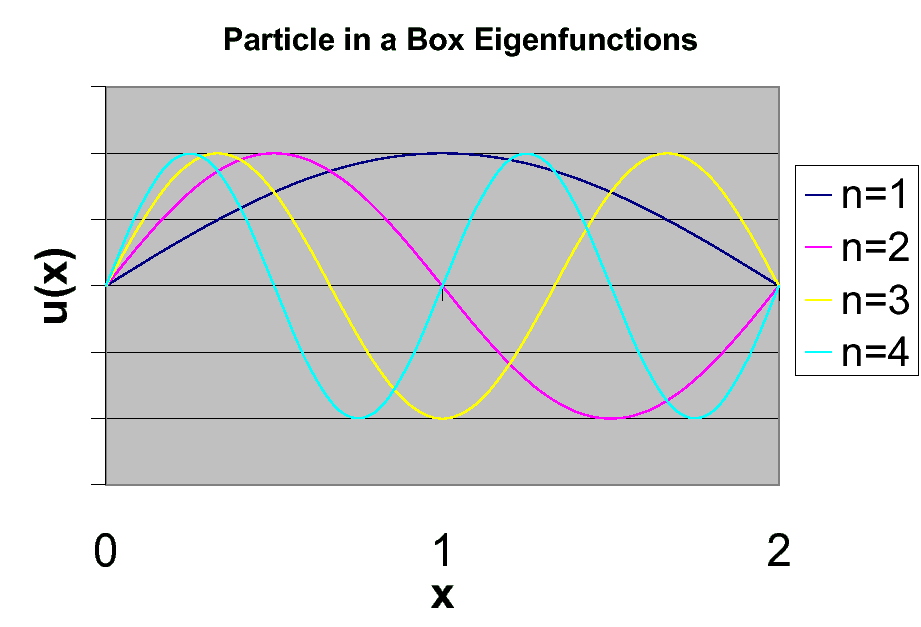
\includegraphics[width=4in]{images/qm/1Dparticle-in-box.png}
    \caption{Particle in Box Wave Function\label{particle-in-box}}
\end{figure}

\subtopic{Postulate 4} 
\hi{Introduce time dependence, equation of motion, and time-dependent Schrodinger equation}



\end{document}
